\documentclass[11pt,a4paper]{article}
\input{../../sablony/pripravy/priprava.sty}
\usepackage{tikz,pgfplots}
\pgfplotsset{compat=1.18}
\nastavPripravu{1. ročník}{Kvadratické rovnice a nerovnice}{113}{Průsečíky kvadratických grafů}
\begin{document}
\blok{Průsečíky kvadratických grafů}
Grafické a algebraické hledání průsečíků dvou parabol; kdy výsledek existuje.
\blok{Metoda a návaznost na graf}
\begin{itemize}
\item Souřadnice společného bodu vyhovují oběma předpisům. Položíme je sobě rovny.
\item Průnik nemusí existovat; při totožných předpisech je společných bodů nekonečně mnoho.
\end{itemize}
\blok{Náčrt před výpočtem}
\begin{center}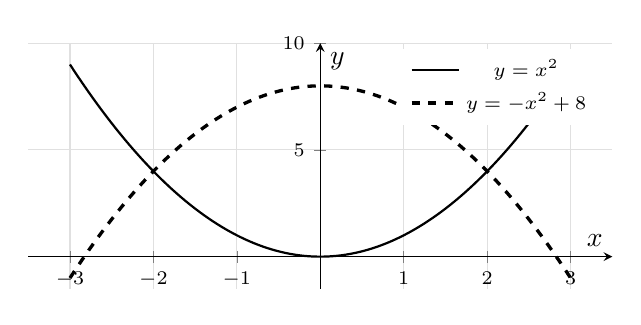
\begin{tikzpicture}
\begin{axis}[width=9cm,height=4.7cm,xmin=-3.5,xmax=3.5,ymin=-1.5,ymax=10,
axis lines=middle,grid=both,grid style={black!12},minor tick num=0,
xlabel={$x$},ylabel={$y$},tick label style={font=\scriptsize},
legend style={font=\scriptsize,draw=none,at={(0.98,0.98)},anchor=north east}]
\addplot[black,thick,domain=-3:3,samples=110] {x^2};\addlegendentry{$y=x^2$}
\addplot[black,dashed,very thick,domain=-3:3,samples=110] {-x^2+8};\addlegendentry{$y=-x^2+8$}
\end{axis}
\end{tikzpicture}\end{center}
\poznamka{Na tabuli nejdříve odhadni počet průsečíků. Algebra následně určí přesné souřadnice.}
\blok{Společně řešené příklady}
\begin{prikladReseniBox}[title={Příklad 1}]
$\begin{cases}y=x^{2}\\y=8 - x^{2}\end{cases}$
\tcblower
\[
\begin{aligned}
x^{2}&=8 - x^{2}\\[2pt]
0&=2x^{2} - 8\\[2pt]
K&=\{[-2;4];\ [2;4]\}
\end{aligned}
\]
\end{prikladReseniBox}
\begin{prikladReseniBox}[title={Příklad 2}]
$\begin{cases}y=x^{2} - 4x + 3\\y=x^{2} - 2x + 1\end{cases}$
\tcblower
\[
\begin{aligned}
x^{2} - 4x + 3&=x^{2} - 2x + 1\\[2pt]
0&=2 - 2x\\[2pt]
K&=\{[1;0]\}
\end{aligned}
\]
\end{prikladReseniBox}
\begin{prikladReseniBox}[title={Příklad 3}]
$\begin{cases}y=x^{2} + 1\\y=- x^{2} - 3\end{cases}$
\tcblower
\[
\begin{aligned}
x^{2} + 1&=- x^{2} - 3\\[2pt]
0&=2x^{2} + 4\\[2pt]
K&=\varnothing
\end{aligned}
\]
\end{prikladReseniBox}
\blok{Samostatné procvičování}
\begin{zadaniReseniBox}[title={Úloha 1}]
$\begin{cases}y=x^{2} + 1\\y=2x^{2} - 3\end{cases}$
\tcblower
\[
\begin{aligned}
x^{2} + 1&=2x^{2} - 3\\[2pt]
0&=4 - x^{2}\\[2pt]
K&=\{[-2;5];\ [2;5]\}
\end{aligned}
\]
\end{zadaniReseniBox}
\begin{zadaniReseniBox}[title={Úloha 2}]
$\begin{cases}y=x^{2} - 1\\y=1 - x^{2}\end{cases}$
\tcblower
\[
\begin{aligned}
x^{2} - 1&=1 - x^{2}\\[2pt]
0&=2x^{2} - 2\\[2pt]
K&=\{[-1;0];\ [1;0]\}
\end{aligned}
\]
\end{zadaniReseniBox}
\blok{Volitelná rezerva}
\poznamka{Studenti si vymyslí obdobný příklad se změnou jednoho koeficientu a vysvětlí, jak se změní počet kořenů či řešení.}
\blok{Volitelná výzva -- průsečíky dvou parabol}
\begin{zadaniReseniBox}[title={Rozšiřující příklad}]
$y=x^2$ a $y=-x^2+8$.
\tcblower
\[\begin{aligned}
x^2&=-x^2+8\\2x^2&=8\\|x|&=2\\K&=\{[-2;4];[2;4]\}
\end{aligned}\]
\end{zadaniReseniBox}
\blok{Domácí úkol}
\begin{zadaniReseniBox}[title={Domácí příprava}]
\begin{enumerate}[label=\alph*),itemsep=2pt]
\item $\begin{cases}y=x^{2} - 4\\y=4 - x^{2}\end{cases}$
\item $\begin{cases}y=x^{2} + 2x + 1\\y=x^{2} - 2x + 1\end{cases}$
\item $\begin{cases}y=2x^{2} - 3\\y=x^{2} + 1\end{cases}$
\item $\begin{cases}y=x^{2} + 5\\y=1 - x^{2}\end{cases}$
\item $\begin{cases}y=x^{2} - 4\\y=0\end{cases}$
\item $\begin{cases}y=x^{2} - 2x + 1\\y=- x^{2} + 2x - 1\end{cases}$
\end{enumerate}
\tcblower
\begin{enumerate}[label=\alph*),itemsep=2pt]
\item
\[\begin{aligned}
x^{2} - 4&=4 - x^{2}\\[2pt]
0&=2x^{2} - 8\\[2pt]
K&=\{[-2;0];\ [2;0]\}
\end{aligned}\]
\item
\[\begin{aligned}
x^{2} + 2x + 1&=x^{2} - 2x + 1\\[2pt]
0&=4x\\[2pt]
K&=\{[0;1]\}
\end{aligned}\]
\item
\[\begin{aligned}
2x^{2} - 3&=x^{2} + 1\\[2pt]
0&=x^{2} - 4\\[2pt]
K&=\{[-2;5];\ [2;5]\}
\end{aligned}\]
\item
\[\begin{aligned}
x^{2} + 5&=1 - x^{2}\\[2pt]
0&=2x^{2} + 4\\[2pt]
K&=\varnothing
\end{aligned}\]
\item
\[\begin{aligned}
x^{2} - 4&=0\\[2pt]
0&=x^{2} - 4\\[2pt]
K&=\{[-2;0];\ [2;0]\}
\end{aligned}\]
\item
\[\begin{aligned}
x^{2} - 2x + 1&=- x^{2} + 2x - 1\\[2pt]
0&=2x^{2} - 4x + 2\\[2pt]
K&=\{[1;0]\}
\end{aligned}\]
\end{enumerate}
\end{zadaniReseniBox}
\poznamka{Orientační čas: úvod 5 min, společné příklady 18 min, samostatně 15 min, kontrola a shrnutí 7 min. Rezerva je dobrovolná. Číselné parametry modelových aplikací nejsou skutečně naměřená data.}
\end{document}
